% !TEX root = ./CM_A-Trabalho.3.tex
\providecommand\mainfilename{"./CM_A-Trabalho.tex"}
\providecommand \subfilename{}
\renewcommand   \subfilename{"./CM_A-Trabalho.3.tex"}
\documentclass[\mainfilename]{subfiles}

% \tikzset{external/force remake=true} % - remake all

\begin{document}

\graphicspath{{\subfix{./.build/figures/CM_A-Trabalho.3}}}
% \tikzsetexternalprefix{./.build/figures/CM_A-Trabalho.3/graphics/}

\mymakesubfile{3}
[CM A]
{Ultilidade} % Subfile Title
{Ultilidade} % Part Title

\begin{sectionBox}1bm{Timeline\cite{Polyurethanes_2022}} % S
    
    \begin{description}[
        leftmargin=!,
        labelwidth=\widthof{} % Longest item
    ]
        \item[1937] Alemanha Descoberto e patentiado por Otto Bayer e colegas
        \item[1940] 2ª Gerra Mundial\par
            Brevemente após a criação esse novo polímero teve grande utilidade como um barata e fácil de obter alternativa a borracha.
            Foi extensivamente utilizado para revestimentos de diversos tipos, desde acabamentos de aviões até uniformes mais resistentes. Foi a primeira introdução de espuma rigida em aviões.
        \item[1941] Adesivos entre borracha, metal e vidro
        \item[1948] Primeiro uso de insulação em um barriu de cerveja.
        \item[1953] Usado como couro sintetico em sólas de sapatos
        \item[1959] Roupas Espaciais\par
            Desenvolvido pela NASA, foi usado como revestimento em trajes espaciais para missões em mercurio
        \item[1967] Alemanha \textit{BMW Bayer K67 "Plastic Car"}\par
            Considerando o primeiro carro completamente feito de plástico no mundo.
            Partes do carro foram feitos usando um novo processo de criação chamado \textit{reaction injection molding} (RIM)
        \item[1973] Patins\par
            Rodas de poliuretano termoplasticos melhoraram e popularizaram patins
        \item[1995] Incluido em rodas de bicicleta para melhorar performance
        \item[1979] Invenção da espuma insulante em spray
        \item[2001] Incluido em rodas de carro para melhorar performance
        \item[2004] Usado nos ventriculos do coração artificial \textit{SynCardia} aprovado para uso clinico
        \item[2008] Pavimento poroso \textit{Elastopave} permite permeabilidade de ar e agua pelo pavimento
        \item[2010] Uso essencial na estrutura do primeiro avião movido a luz solar a voar ao redor do planeta
        \item[2011] Primeira planta que manufatura poliuretano a partir de dioxido de carbono aberta na Alemanha
    \end{description}
\end{sectionBox}

\begin{sectionBox}1bm{Breakdown das propriedades\cite{Polyurethanes_2022}} % S
    
    Poliuretano é composto por isocianatos (em excesso) e poliols, normalmente na presença de catalizadores ou esposição a ultra violeta. A variação dos seus compostos e quão densa é formada a espuma (usando agentes de expansão) podem ser explorados para preparar um material que se encaixa nas mais variadas funções e necessidades.\par
    \begin{sectionBox}*b{} % S
        \paragraph*{Densidade da espuma\cite{Polyurethanes_2022}}
        \begin{description}[
            leftmargin=!,
            labelwidth=\widthof{} % Longest item
        ]
            \item[Baixa] Uso comum de dioxido de carbono como agente extensor para criar uma espuma macia e confortável, comumente usado em sofás ou camas.
            \item[Média] Em espumas rigidas, prendendo gáses como pentano optimiza propriedades de insulação
            \item[Alta] Não usando nenhum agente expansor resulta numa estrutura de consistencia densa e resiliente que foi usada em rodas de patins por exemplo.
        \end{description}
    \end{sectionBox}

    \begin{sectionBox}2bm{Isocianatos\cite{americanchemistry}} % S
        Costumam ser divididos em dois tipos: aromáticos e aliphaticos, onde os primeiros são muito mais comunmente usados.\par
        Os Isocianatos aromáticos se dividem (majoritariamente) em duas categorias tolueno diisocianato (TDI) e metilenodifeil diisocianato (MDI):
        \begin{center}
            \schemestart
                \chemname{\chemfig{
                    [:150]*6(=-=(-NCO)-=-)
                    -[:0]CH2
                    -[:0]*6(=-=(-NCO)-=-)
                }}{4,4'-diphenylmenthane diisocyanate (MDI)}
                \chemname{\chemfig{
                    NCO-[:90]*6(
                        =-(-NCO)=(-CH3)-=-
                    )
                }}{2,4 - toluene diisocyanate (TDI)}
            \schemestop
        \end{center}
        \begin{multicols}{2}
            \begin{sectionBox}3bm{MDIs} % S
                
                São divididos em duas formas: MDI puros e MDI Polimétricos (pMDI). Quando usados na produção de espumas de poliuretanos garantem \emph{maior rigidez e propriedades isolantes}, essas espumas são bastante aplicadas no \emph{isolamento de casas e refrigeradores} garantindo menor consumo energético tambem podemos encontrar em \emph{sólas de sapatos}.
            \end{sectionBox}
            \begin{sectionBox}3bm{TDI} % S
                
                Os TDIs são primariamente usados para produção de espumas \emph{flexiveis e léves}, essas são usadas na \emph{fabricação de móveis, roupas de cama e revestimento de automóveis}.
                Em aplicações no transporte garante \emph{peças mais leves} aumentando a eficiencia energética.
                
            \end{sectionBox}
        \end{multicols}
        
    \end{sectionBox}

    \begin{sectionBox}2bm{Peças de automóveis} % S
        
        \begin{center}
            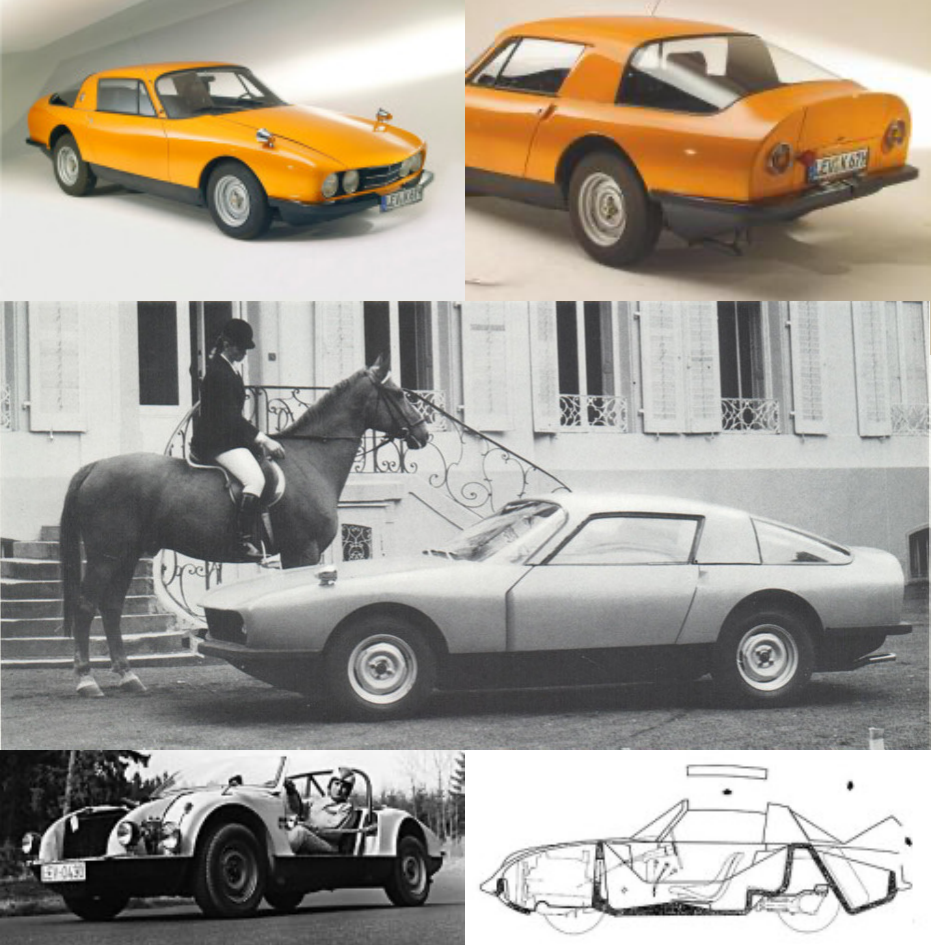
\includegraphics[width=.9\textwidth]{plasticarcollage.png}
            \captionof{figure}{Compilação de fotods do \textit{Bayer's All plastic car}, tambem conhecido como o \emph{carro de poliuretano}, foi o primeiro carro feito completamente de plástico no mundo, poliuretano foi extensamente usado na composição das peças\cite{hatari007_2017}}
        \end{center}
        
    \end{sectionBox}

    \begin{sectionBox}2bm{Isolamento de casas e refrigeradores} % S
        
        \subsubsection{Spray de Poliuretano (SPF)\cite{SPF}}
        Dois liquidos combinam para reagir e formar o SPF no momento que ele é expelido pelo spray, esses dois liquidos vem em diferentes containers geralmente referidos por proficionais como parte ``A'' composto de MDI e pMDI e parte ``B'' composto de um blend de poliols, catalizadores, agente expansor, retardador de chama e surfactante.
        \paragraph*{Nota:} Os lados ``A'' e ``B'' podem se reverter fora dos estados unidos.
        Esta é uma aplicação bastante utilizada por sua versabilidade superar a menor qualidade do material comparado com outros isolantes, os barris podem ser trazidos para a construção e a reação ser feita diretamente nas paredes permite acomodar qualquer forma alem de ocupar uma area muito maior como espuma do que como reagentes.
        \begin{center}
            \includegraphics[width=.8\textwidth]{SPF.jpg}
            \captionof{figure}{Aplicação do SPF na parte interna de paredes em construções\cite{SPFImage}}
        \end{center}
        \subsection{Isolamento de freesers\cite{WhirlpoolRefrigerators}}
        Em 2012 foi comercializada por Whirlpool Corp. o primeiro freezer que usa como isolante a espuma de poliuretano usando como agente extensor HFO (Hidrofluorolefinas).
        
    \end{sectionBox}

    \begin{sectionBox}2bm{Couro de Poliuretano (PU Leather)} % S
        
        \paragraph*{1950 -- Sneackers\cite{Foster_2021}}
        Nessa época vários móveis e roupas que faziam uso de couro ou borracha vulcanizada passaram a usar o couro artificial, reduzindo o preço de produção. 
        \begin{center}
            \includegraphics[width=.6\textwidth]{screen-shot-2016-01-05-at-14.47.05.png}
            \captionof{figure}{Propaganda de Sneakers em 1950 que utilizavam PU Leather\cite{Foster_2021}}
        \end{center}
        
    \end{sectionBox}
    
\end{sectionBox}

\end{document}